\documentclass[11pt]{article}

% Load packages
\usepackage{amsthm,amsmath,amssymb}
\usepackage{dsfont}
\usepackage{graphicx}
\usepackage{natbib}
\usepackage[colorlinks,citecolor=blue,urlcolor=blue]{hyperref}
\usepackage[utf8]{inputenc}
\usepackage[margin = 2.5cm]{geometry}
\usepackage{booktabs}
\usepackage{float}

\usepackage{tikz}
\usetikzlibrary{shapes,decorations,arrows,calc,arrows.meta,fit,positioning}
\tikzset{
	-Latex,auto,node distance =1 cm and 1 cm,semithick,
	state/.style ={ellipse, draw, minimum width = 0.7 cm},
	point/.style = {circle, draw, inner sep=0.04cm,fill,node contents={}},
	bidirected/.style={Latex-Latex,dashed},
	el/.style = {inner sep=2pt, align=left, sloped}
}

\usepackage{sectsty}
\sectionfont{\fontsize{12}{16}\selectfont\centering}
\subsectionfont{\fontsize{11}{14}\selectfont}

\usepackage{hyperref}
\hypersetup{colorlinks,linkcolor={blue},citecolor={blue},urlcolor={blue}}  

% define helper commands
\newcommand{\E}{\mathbb{E}}
\newcommand{\Prob}{\mathbb{P}}


% Title Page
\title{The Impact of Natural Disasters on Education: \\ Evidence from Standardized Testing}
\author{Gregor Steiner}


\begin{document}
\maketitle

\begin{abstract}
	\centering
	\begin{minipage}{\dimexpr\paperwidth-10cm}
		The frequency and severity of natural disasters has increased recently, but we do not fully understand the impacts. We use an event-study design to estimate dynamic treatment effects of natural disasters on students' performance in standardized tests. There is a significant effect on the performance in mathematics in the period of the disaster. For achievement in Reading Language Arts we find no significant effect. Furthermore, we find a significantly negative effect of extreme heat exposure on standardized test scores for some groups.
	\end{minipage}
\end{abstract}


% sections

\section{Introduction}

Natural disasters are responsible for massive economic damage and due to climate change the frequency of such disasters will increase in most regions \citep{IPCC_2021}. Therefore, it is essential to have a good understanding of the consequences. While much research has been done on the macroeconomic consequences of natural disasters, few studies have focused on the impact on education. This study investigates the effect of natural disasters on academic performance.

A causal effect of natural disasters may be driven by school closures \citep{Grewening_2020}, destroyed infrastructure, and emotional stress \citep{Vogel_2016}. Furthermore, some forms of natural disasters, e.g. extreme heat, may directly impair cognitive performance \citep{Ramsey_1995}.

To identify dynamic causal effects of experiencing natural disasters, this paper uses an event-study design. In particular, we estimate dynamic treatment effects for up to eight years after initial treatment. As a result, not only short-term but also medium to long-term effects can be found. Since treatment effects are likely very heterogenous, we use the estimator by \cite{Sun_2021}. 

This article uses standardized test data on a US county level for grades 3 through 8 in mathematics and reading language arts (RLA) to measure academic performance, covering the school years 2008/2009 to 2018/2019. This measure is very attractive as the test scores are standardized relative to a national reference cohort. Therefore, the outcomes are nationally comparable. For the same period, we obtain data on natural disasters from declarations by the Federal Emergency Management Agency and data on storms from the National Weather Service.

This article contributes to a rich literature on economic effects of natural disasters. More specifically, this paper contributes to the literature on the impact of natural disasters on education. Previous work has produced mixed results. Some authors find significant effects of natural disasters on the education system \citep{Holmes_2002, Cuaresma_2010, Sacerdote_2012, Goodman_2020}, while others find no or only small effects \citep{Baggerly_2008, Pane_2008}. Morover, some authors find large differences by subject \citep{Spencer_2016}.

Previous studies have concentrated on a single type, or even a single instance of disasters. For example, hurricane Katrina has been the subject of many studies \citep[e.g.][]{Sacerdote_2012, Deryugina_2018}. To the best of our knowledge, this is the first study to exploit a very comprehensive dataset of natural disasters, including various different types of disasters. 

The rest of this paper is organized as follows: Section \ref{Data} introduces the data used and presents some descriptive statistics. Section \ref{EmpStrat} explains the empirical strategy. Section \ref{Results} discusses the results and section \ref{Conclusion} concludes.




\section{Background \& Data} \label{Data}

\subsection{Natural Disasters in the United States}

Natural disasters cause numerous fatalities and billions of dollars of infrastructure damage in the United States each year \citep{Boustan_2020}. With more greenhouse gas in the atmosphere the number and severity of such disasters will increase \citep{IPCC_2021}. Figure \ref{DisasterCount} shows the number of county-level disasters per year. However, note that a single disaster that affects multiple counties counts as multiple county-level disasters. The majority of natural disasters in the US is made up by storms, such as hurricanes or tornadoes, floodings, and fires. Some well-known examples include the 2020 wildfire season in the western United States, Hurricane Harvey in 2017, or Hurricane Katrina in 2005.

\begin{figure}[!h]
	\centering
	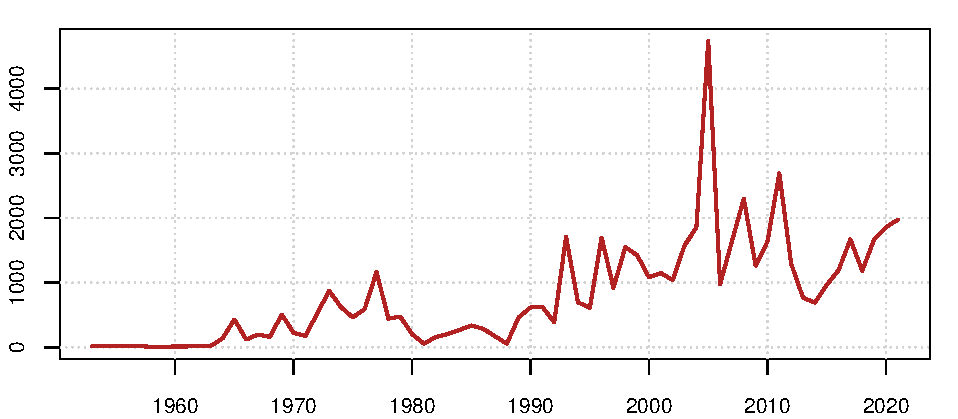
\includegraphics[scale=1]{"../Code & Data/DisasterCount.pdf"}
	\caption{Number of county-level natural disasters by year}
	\label{DisasterCount}
\end{figure}

The handling of natural disasters is governed by the \cite{Stafford}. It defines major disasters as follows:
\begin{quote}
	 Major disaster means any natural catastrophe (including any 	hurricane, tornado, storm, high water, winddriven water, tidal wave, tsunami, earthquake, volcanic eruption, landslide, mudslide, snowstorm, or drought), or, regardless of cause, any fire, flood, or explosion, in any part of the United States, which in the determination of the President causes damage of sufficient severity and magnitude to warrant major disaster assistance under this Act to supplement the efforts and available resources of States, local governments, and disaster relief organizations in alleviating the damage, loss, hardship, or suffering caused thereby.
\end{quote}
Based on the Stafford Act major disaster declarations are made solely by the president upon request by the affected state's governor. State officials must prove that the situation is beyond the capabilities of the state governemnt or involved local governments. The Federal Emergency Management Agency (FEMA) evaluates requests for major disasters and makes recommendations to the president.

A major disaster declaration provides a wide range of federal assistance programs for individuals and public infrastructure, including funds for both emergency and permanent work. In particular, affected state and local governments can receive federal disaster assistance as part of the Public Assistance program, while individuals and households can receive aid from the Individual Assistance program. Moreover, State, Tribal, and local governments and certain private nonprofit organizations can receive assistance for preventive actions taken based on the Hazard Mitigation Assistance program.

FEMA provides data on all federally declared natural disasters, beginning in 1953. The data is easily accessible via their API \citep{rfema}. This is the main source for natural disaster data used here. Figure \ref{DisasterMap} shows the number of declared disasters between 2009 and 2018 across the US. Table \ref{DisasterTypes} shows the types of disasters and their proportion in the FEMA data. Storms make up the largest share of disaster events. Fires and floods also form a substantial part.

\begin{figure}[!h]
	\centering
	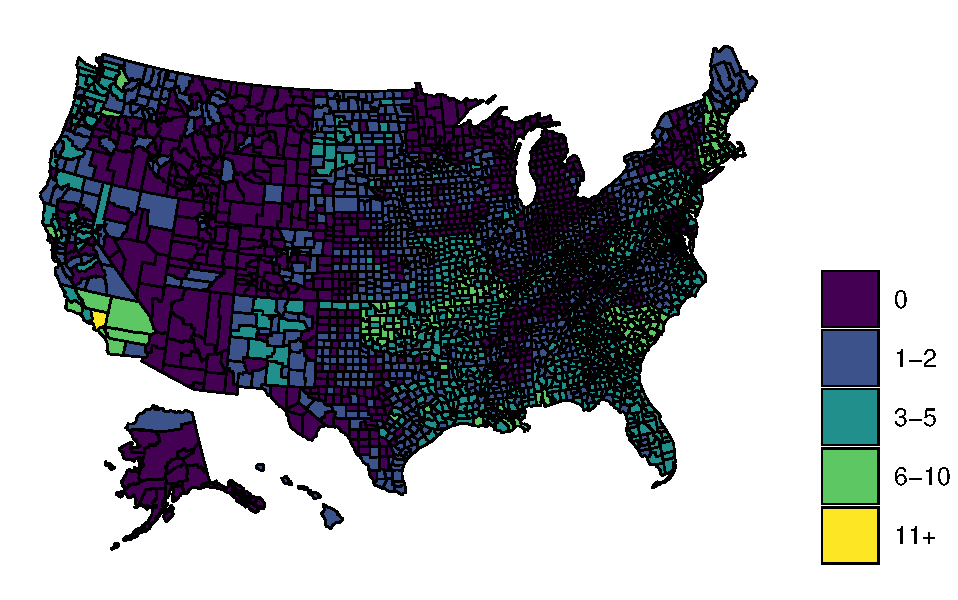
\includegraphics[scale=1]{"../Code & Data/DisasterMap.pdf"}
	\caption{Number of declared natural disasters in school years 2008-09 through 2017-18}
	\label{DisasterMap}
\end{figure}

\begin{table}[!h] \centering \caption{Disasters from 2009 to 2018 by type}\label{DisasterTypes}
\begin{tabular}{lrr}
\hline
\hline
Variable & N & Percent \\ 
\hline
Disaster Type & 13230 &  \\ 
... Chemical & 9 & 0.1\% \\ 
... Coastal Storm & 12 & 0.1\% \\ 
... Dam/Levee Break & 3 & 0\% \\ 
... Earthquake & 19 & 0.1\% \\ 
... Fire & 886 & 6.7\% \\ 
... Flood & 2006 & 15.2\% \\ 
... Freezing & 1 & 0\% \\ 
... Hurricane & 3094 & 23.4\% \\ 
... Mud/Landslide & 28 & 0.2\% \\ 
... Other & 7 & 0.1\% \\ 
... Severe Ice Storm & 803 & 6.1\% \\ 
... Severe Storm(s) & 5644 & 42.7\% \\ 
... Snow & 577 & 4.4\% \\ 
... Terrorist & 4 & 0\% \\ 
... Tornado & 114 & 0.9\% \\ 
... Toxic Substances & 1 & 0\% \\ 
... Tsunami & 9 & 0.1\% \\ 
... Typhoon & 11 & 0.1\% \\ 
... Volcano & 2 & 0\%\\ 
\hline
\hline
\end{tabular}
\end{table}



We repeat the analysis on two different datasets: Data on storms and data on heat exposure. First, this acts as a robustness check. These two datasets are based on obective measurements, while the FEMA data is based on subjective declarations. Second, this allows us to better understand heterogeneity by type of disaster.

The National Weather Service (NWS) provides data on storm events. In particular, this covers hurricanes, tornadoes, and other severe storms. These make up a very large part of all natural disasters experienced in the United States (see table \ref{DisasterTypes}). Combined they account for more than 80\% of all disaster damage in the FEMA Public Assistance Applicants Program Deliveries database.

\begin{figure}[!h]
	\centering
	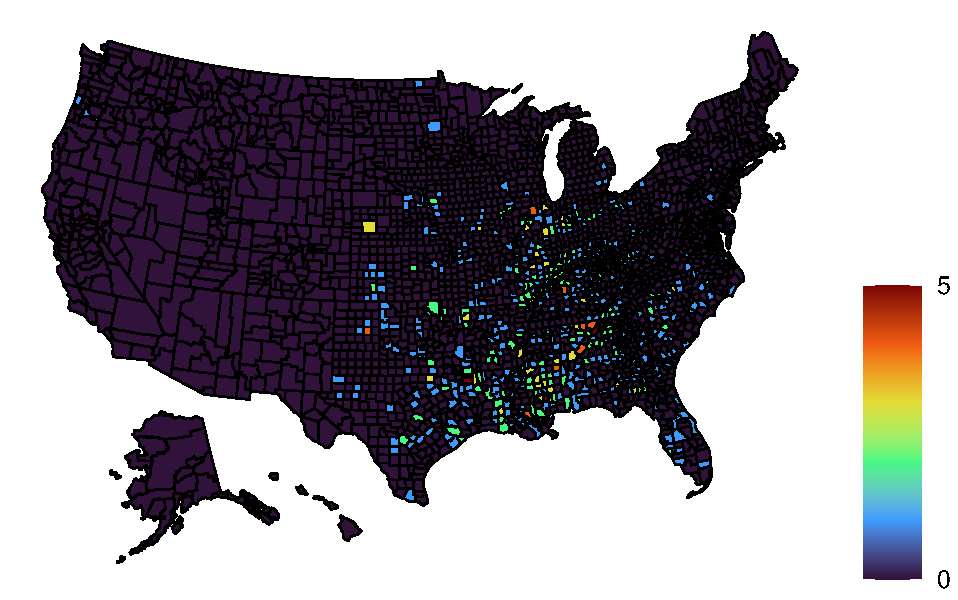
\includegraphics[scale=1]{"../Code & Data/StormMap.pdf"}
	\caption{Number of storms in school years 2008-09 through 2017-18}
	\label{StormMap}
\end{figure}

We only consider severe storms which are likely to cause substantial damage. Tornadoes can be classified based on estimated peak wind speeds on the Enhanced Fujita (EF) scale \citep[for more details see][]{EF_Scale}. Tornadoes with an EF scale of 0 or 1 (wind speeds of up to 110 mph) are characterized as weak. Therefore, we exclude those and only keep tornadoes with an EF scale of at least 2 (wind speeds of at least 111 mph). Unfortunately, the hurricane data does not include a similar measure, but it does include an estimated amount of property damage. We exclude all hurricanes with an estimated property damage of zero.  Storm exposure by county is shown in figure \ref{StormMap}.

To measure heat exposure, we exploit daily temperature data from the Global Historical Climatology Network \citep{Menne_2012}. Each county is assigned the measurement station with the lowest distance to the county's center. Following \cite{Goodman_2020}, we use two measures of yearly cumulative heat exposure: The average daily maximum temperature and the number of days with a maximum temperature above 30°C in a school year. The threshold of 30°C is somewhat arbitrary, however, changing it slightly does not change the results in a meaningful way. Figures \ref{HeatMapTemp} and \ref{HeatMapDays} show the distribution across counties. As expected, the variation in heat exposure is largely driven by location.

\begin{figure}[!h]
	\centering
	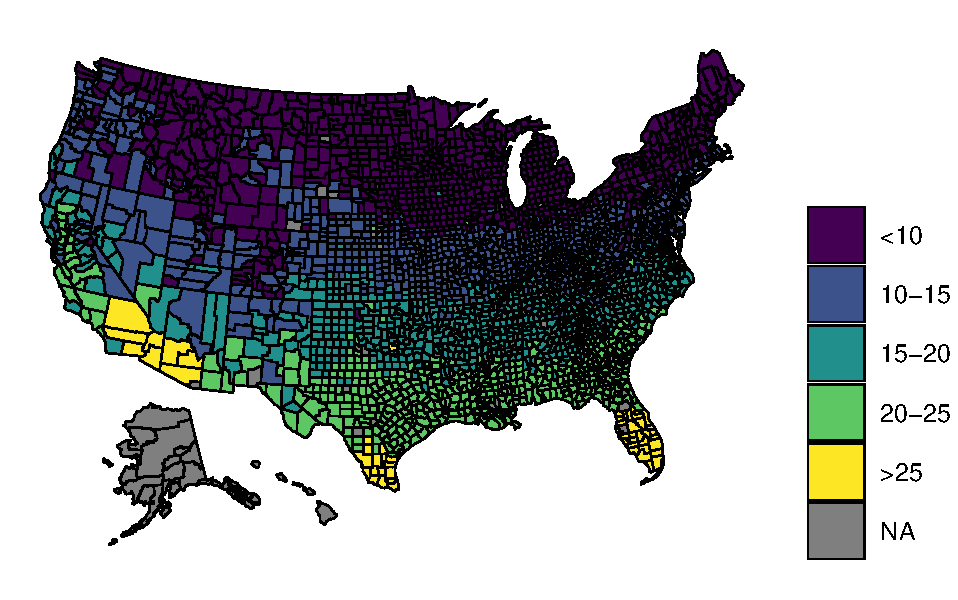
\includegraphics[scale=1]{"../Code & Data/HeatMapTemp.pdf"}
	\caption{Average daily maximum temperature (in °C) in school years 2008-09 through 2017-18}
	\label{HeatMapTemp}
\end{figure}

\begin{figure}[!h]
	\centering
	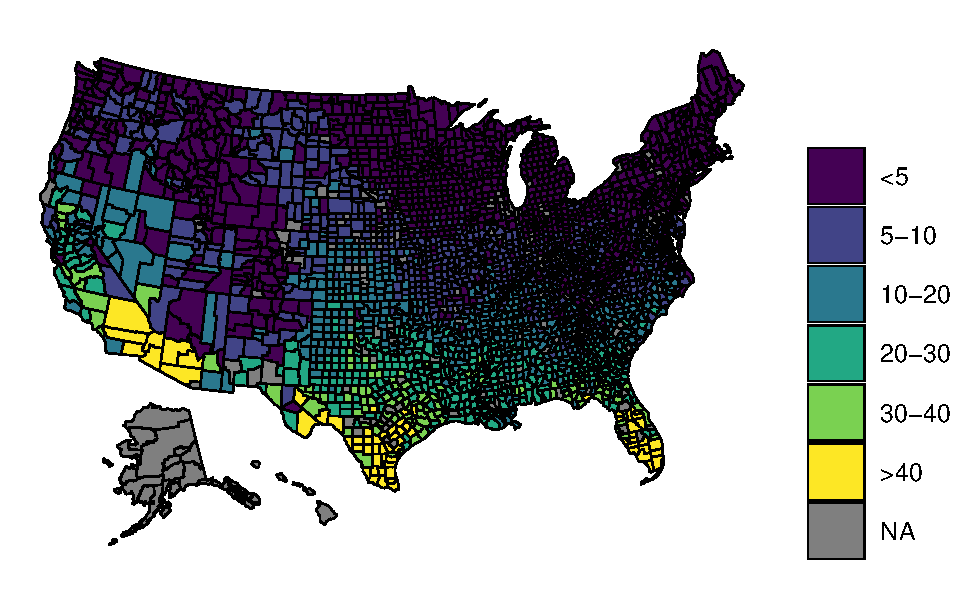
\includegraphics[scale=1]{"../Code & Data/HeatMapDays.pdf"}
	\caption{Average number of days above 30°C in school years 2008-09 through 2017-18}
	\label{HeatMapDays}
\end{figure}


\subsection{Assistance Applications}

After severe disasters counties frequently receive public assistance. This potentially creates a selection problem: The counties receiving state aid are likely coping better with the consequences of the natural disaster. If the assignment of federal aid is not independent of the disaster's consequences, this creates a problem for our identification. Since assistance provision is at least somewhat dependent on disaster severity, this is very probable.

FEMA provides a dataset on  their Public Assistance Applicants Program Deliveries. It contains information on applicants and their recovery priorities, including the amount of damage caused and amount of federal disaster assistance granted. This is the main program for federal public disaster assistance, averaging USD 4.7 billion in assistance each year. However, note that counties that do not receive public assistance may still benefit from individual assistance or from the Hazard Mitigation Assistance program.

Unfortunately, this data is only available starting in October 2016. Based on the temporal overlap between this dataset and our main dataset, that is schoolyears 2016/2017 and 2017/2018, it is possible to analyze whether counties that are affected by disasters receive federal assistance. This can be done by checking whether a county that experienced a disaster in 2016/2017 or 2017/2018 appears in the Public Assistance Applicants Program Deliveries database. In fact, only about 17.78\% of counties that experienced a disaster in that period did apply for federal assistance. Table \ref{tab:AppsByType} shows the number of disasters and the share of counties that applied for assistance following such a disaster by disaster type. It seems that the number varies dramatically by disaster type. While about 80\% of counties affected by a tornado applied for federal assistance, only about 10\% of counties affected by fires or floods did so.

\begin{table}

\caption{\label{tab:AppsByType}Share of counties that applied for federal assistance following a disaster by disaster type (schoolyears 2016-17 and 2017-18)}
\centering
\begin{tabular}[t]{lrr}
\toprule
  & Number of Cases & Applied for Assistance (in \%)\\
\midrule
Coastal Storm & 3 & 33.33\\
Dam/Levee Break & 3 & 0.00\\
Fire & 100 & 11.00\\
Flood & 270 & 41.85\\
Hurricane & 1217 & 23.25\\
Mud/Landslide & 22 & 50.00\\
Severe Ice Storm & 20 & 0.00\\
Severe Storm(s) & 164 & 28.66\\
Snow & 36 & 8.33\\
Tornado & 29 & 79.31\\
\addlinespace
Total & 1864 & 26.39\\
\bottomrule
\end{tabular}
\end{table}


It may be interesting to see how these counties differ from the ones that did apply. Figure \ref{AssistCovBoxplot} shows boxplots by county application status. Counties that did apply for federal disaster assistance tend to have lower median income, higher poverty rates, and higher shares of single motherhood. Thus, it seems that counties that had to apply for federal disaster assistance were more socially vulnerable in the first place. This is consistent with the findings in \cite{Gao_2022}.

However, the direction of causality is not clear. Possibly these counties are more frequently affected by natural disasters and are also poorer or more socially vulnerable because of it. Alternatively, counties that are poorer could be more likely to apply for public disaster aid as they have fewer private resources. While there is some correlation between disaster risk and economic conditions \citep[for example][]{Goodman_2020}, the latter explanation seems more likely overall.

\begin{figure}[!h]
	\centering
	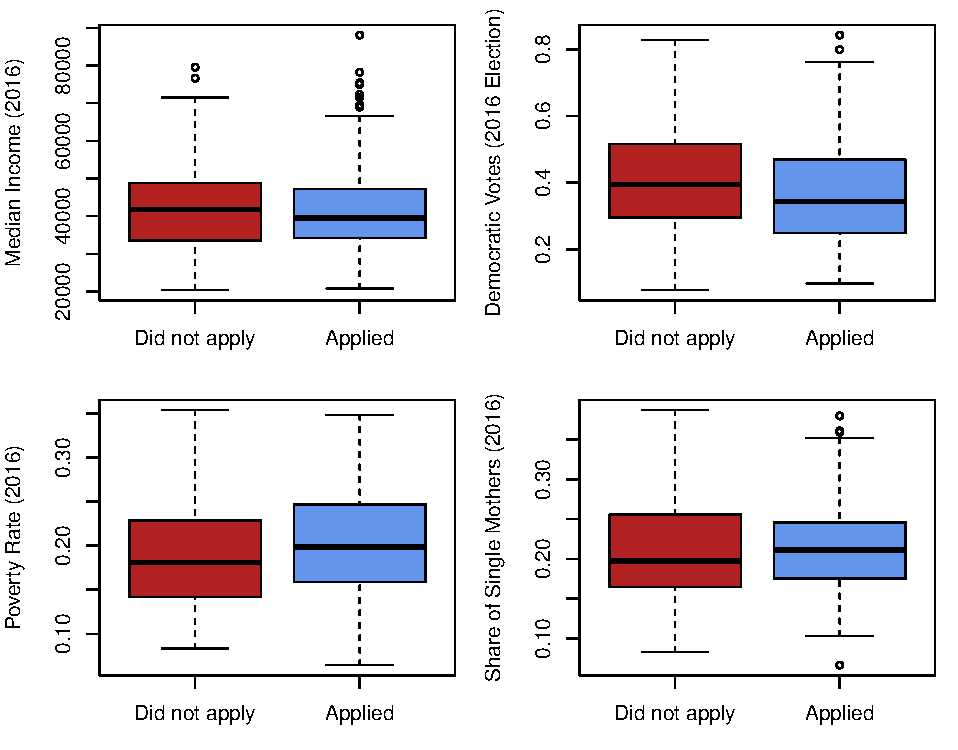
\includegraphics[scale=1]{"../Code & Data/AssistanceCovBoxplot.pdf"}
	\caption{Boxplots by application status}
	\label{AssistCovBoxplot}
\end{figure}

It is also interesting whether variation in the federal assistance procedure may be driven by political factors. Visually, democratic votes in the 2016 election (almost coincides with the start of the Public Assistance Applicants Program Deliveries dataset) tend to be lower in counties that applied. That is, counties that applied for federal assistance tend to vote more Republican. Logistic regression results confirm the visual impression (see Appendix \ref{AppendixA}). While this is not necessarily a causal effect, it could be an indication that a Republican president may be more hesitant awarding disaster assistance to Democratic counties.

There are clear differences between counties that receive federal assistance after a disaster and counties that do not. This is a potential problem to the identification of a causal effect. However, counties that are severely affected and receive assistance would most likely experience even worse consequences, did they not receive assistance. Thus, our estimates may only be a lower bound for the negative effect.


\subsection{Standardized Testing Data}

Data on academic achievement is available from the Stanford Education Data Archive \citep{SEDA}. They provide mean test results from standardized tests by county, year, grade and subject among all students and various subgroups (including race, gender, and economically disadvantaged). The most recent version 4.1 covers grades 3 through 8 in mathematics and Reading Language Arts (RLA)\footnote{RLA assesses students' ability to understand what they read and to write clearly.} over the 2008-09 through 2017-18 school years.

Test scores are cohort-standardized, meaning they can be interpreted relatively to an average national reference cohort in the same grade. This makes the dataset very attractive, as test scores are nationally comparable. For instance, a county mean of 0.5 indicates that the average student in the county scored approximately one half of a standard deviation higher than the average national student in the same grade.

In addition to overall mean test scores, the data includes mean test scores for various subgroups, e.g. by ethnicity. In particular, we consider mean test scores for white, black, hispanic, female, and economically disadvantaged students to investigate whether the effects differ by ethnicity, gender, or socioeconomic position. These are only reported if the subgroups' sample sizes are large enough to guarantee anonymization. Thus, the number of observations for some of the groups is substantially smaller.

The outcomes of interest are overall mean test scores by county, and mean test scores for white, black, hispanic, female, and, economically disadvantaged students. Figure \ref{DepVarsBoxplot} shows boxplots for the five outcomes of interest and Table \ref{tab:SumStats} provides summary statistics. Due to the way the scale is constructed, overall test scores are distributed symmetrically around zero, except for a few outliers. The mean scores for black, hispanic, and economically disadvantaged students tend to be lower than the overall means, while white students tend to perform slightly better than the overall average. Female mean scores are slightly above overall mean scores, meaning that female students perform slightly better than male students on average.

\begin{table}

\caption{\label{tab:SumStats}Summary statistics for dependent variables}
\centering
\begin{tabular}[t]{lrrrrrr}
\toprule
  & Overall & White & Black & Hispanic & Female & Econ. disadv.\\
\midrule
Mean & -0.042 & 0.107 & -0.483 & -0.281 & 0.025 & -0.284\\
Std. Dev. & 0.294 & 0.262 & 0.273 & 0.266 & 0.295 & 0.256\\
Min. & -3.196 & -2.936 & -2.745 & -1.699 & -2.862 & -3.007\\
Max. & 1.669 & 1.700 & 1.394 & 1.374 & 1.496 & 1.312\\
\bottomrule
\end{tabular}
\end{table}


\begin{figure}[!h]
	\centering
	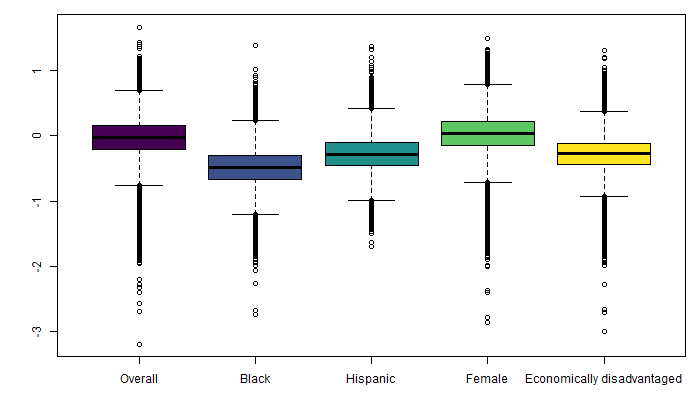
\includegraphics[scale=1]{"../Code & Data/DepVarsBoxplot.pdf"}
	\caption{Boxplots of the outcomes of interest}
	\label{DepVarsBoxplot}
\end{figure}


Natural disasters should only have an effect on test scores if they occur before the test. Standardized tests are generally administered in March, April, or May. We will use March 1st as a cut-off point. Thus, any disaster happening within the same school year before the 1st of March will be considered. School years tend to start in late August or early September with some variation across states. We will use September 1st, meaning any disaster happening between September 1st and March 1st will be counted for a given school year. Disasters occuring in the summer or in the spring after the exams should have much less influence on performance. Thus, we do not consider disasters that occur between March 1st and September 1st.

Each disaster is assigned to a school year as described above. Then, disaster and test score data can be merged by school year and county. This yields a panel data set with six grades and two subjects for each county-year combination.




\section{Empirical Strategy}

\subsection{Setting}

We employ an event study design to measure the effect of natural disasters on standardized test outcomes. An event study design is a staggered adoption design where units are first-treated at different points in time, and there may or may not be never-treated units \citep{Sun_2021}.

In order to identify a causal effect, unobservable determinants of a county's test scores must be unrelated to natural disasters conditional on observable characteristics of that county. The occurrence of natural disasters is plausibly random conditional on location. Furthermore conditioning on the year should account for an increasing trend in natural disasters due to climate change. Thus, independence of mean test scores and natural disasters is plausible conditional on county and year fixed effects.

Consequently, the baseline specification is
\begin{align} \label{baseline}
	y_{i, t, g} = \sum_{l = -9, l \neq -1}^{8} \beta_l D_{i, t-l} + \alpha_i + \lambda_t + \zeta_g + X_{i, t} \gamma + \varepsilon_{i, t, g} \;,
\end{align}
where $y_{i, t, g}$ is the outcome of interest for county $i$, year $t$, and grade $g$. County, year, and grade fixed-effects are given by $\alpha_i$, $\lambda_t$, and $\zeta_g$ respectively and $X_{i, t}$ is a row vector of additional control variables. $D_{i, t-l}$ is a treatment indicator for county $i$ in year $t-l$. That is, $D_{i, t-l} = 1$ if the county had already experienced a disaster $l$ years ago at time $t$.

Since we consider the time period 2009-2018, $-9 \leq l \leq 9$, but note that $l = 9$ would correspond to a unit that experienced a disaster in the first period and is therefore always treated. As recommended by \cite{Sun_2021}, these units are dropped from estimation, since no treatment effects can be identified for that group\footnote{At least not under standard assumptions. If one is willing to make assumptions about the trends of both potential outcomes, then it may make sense to keep always treated units \citep[see][]{Marcus_2021}, but this is not the case here.}.

Also, we need to drop at least two leads or lags to avoid a multicollinearity problem. A complete set of treatment leads and lags is perfectly collinear with unit and time fixed-effects \citep[for an extensive discussion of this issue see][section 3.2]{Borusyak_2021}. It is common to drop the first relative indicator prior to treatment (i.e. $\beta_{-1} = 0$). This acts as a normalization of treatment relative to the period before treatment. Furthermore, we bin the distant leads, that is we combine the treatment indicators for $l \leq -5$. Thus, equation (\ref{baseline}) turns into
\begin{align} \label{baselineBinned}
	y_{i, t, g} = \beta_{-5} \sum_{l \leq -5} D_{i, t-l} + \sum_{l = -4, l \neq -1}^{8} \beta_l D_{i, t-l} + \alpha_i + \lambda_t + \zeta_g + X_{i, t} \gamma + \varepsilon_{i, t, g} \;.
\end{align}
Note that treatment must be absorbing, meaning the sequence $(D_{i, t})_{t=1}^T$ must be a non-decreasing sequence of $0$s and $1$s. In other words, after being treated for the first time a county stays treated. In the present application this means treatment refers to having experienced a disaster rather than experiencing a disaster in that year. This is common practice and does not cause bias due to the conditionally random nature of natural disasters \citep{Deryugina_2017}. Thus, the emphasis lies on cumulative long-term effects rather than instantaneous short-term effects.

It is implausible that the treatment effects are constant in our setting. The extent of disasters varies substantially, and also the level of preparation for such disasters likely displays high variance across counties. 

\subsection{Interaction-weighted estimator}

We utilize the interaction-weighted (IW) estimator proposed by \cite{Sun_2021} that is robust to treatment effects heterogeneity. The main interest lies on the cohort average treatment effect on the treated (CATT),
\begin{align*}
	CATT_{e, l} := \E \left[ Y_{i, t+l} - Y_{i, t+l}^{\infty} | E_i = e \right],
\end{align*}
where $Y_{i, t+l}^{\infty}$ is the counterfactual of being never treated and $E_i$ denotes the first treatment period. Thus, $CATT_{e, l}$ is the average treatment effect on the treated $l$ years after being treated for the first time for the cohort that was first treated in year $e$.

The estimation procedure consists of three main steps:
\begin{enumerate}
	\item Estimate $CATT_{e, l}$ using a linear fixed effects specification with interactions between relative period indicators and cohort indicators:
	\begin{align} \label{CATTDID}
		y_{i, t, g} = \sum_{e \notin C}^{}\sum_{l \neq -1}^{} \delta_{e, l} (\mathds{1}\{E_i = e\} D_{i, t-l}) + \alpha_i + \lambda_t + \zeta_g + \varepsilon_{i, t, g} \;,
	\end{align}
	where $C$ is the set of comparison cohorts. In our case $C$ is the never treated cohort, i.e. $C = {\infty}$. If there is a cohort that is always treated, i.e. that already receives treatment in the first period, then we need to exclude this cohort. The coeffiecient estimator $\widehat{\delta}_{e, l}$ that we obtain from (\ref{CATTDID}) estimates $CATT_{e, l}$.
	
	\item Weight the estimators by the share of the respective cohort in the sample in that period. Let $\hat{W}^l$ be a weight matrix with element $(t, e)$
	\begin{align*}
		[\widehat{W}^l]_{t, e} := \frac{\mathds{1}\{t - e = l\} \sum_{i = 1}^{N} \mathds{1}\{E_i = e\}}{\sum_{e \in h^{l}} \sum_{i = 1}^{N} \mathds{1}\{E_i = e\}},
	\end{align*}
	where $h^{l} := \{e: 1 - l \leq e \leq \max(E_i) - 1 - l\}$ is the set of cohorts that experience at least $l$ periods of treatment.
	
	\item Take the average over all $CATT_{e, l}$ estimates weighted by the cohort shares in the weight matrices. Let $vec(A)$ be the vectorize operator that vectorizes matrix $A$ by stacking its columns and let $\widehat{\delta}$ be the vector that collects $\widehat{\delta}_{e, l}$ for all $e$ and $l$. Then, the IW estimator $\widehat{v}_g$ for bin $g$ can be written as 
	\begin{align}
		\widehat{v}_g := \frac{1}{|g|} \sum_{l \in g} [vec(\widehat{W}^l)]^\intercal \widehat{\delta}.
	\end{align}
	For a singleton bin $g = \{l\}$, this simplifies to
	\begin{align*}
		\widehat{v}_{g} := [vec(\widehat{W}^l)]^\intercal \widehat{\delta}.
	\end{align*}
	
\end{enumerate}

Under some standard assumptions, $\widehat{v}_g$ is asymptotically normal \citep[for a proof and a detailed description of said assumptions see][Appendix C]{Sun_2021}. Under the additional assumptions of parallel trends and no anticipatory behavior, $\widehat{v}_g$ is consistent, that is it converges in probability to
\begin{align*}
	\widehat{v}_g \overset{p}{\to} [vec(W^{l})]^\intercal \delta = \sum_{e \in h^{l}} \Prob(E_i = e | E_i \in h^{l}) CATT_{e, l} \; ,
\end{align*}
where $W^{l}$ is the probability limit of the weight matrix $\widehat{W}^l$.


We use the existing implementation in the \textbf{fixest} R package \citep{Berge_2018}.

\subsection{Identifying assumptions}

Below we discuss the identifying assumptions.

\textbf{Parallel Trends:} Parallel trends in the sense of \cite{Sun_2021} refers to the following: $\E[Y_{i, t}^{\infty} - Y_{i, s}^{\infty} | E_i = e]$ does not depend on $e$ for any $s \neq t$. That is, the expected temporal difference, i.e. the trend, in the potential outcomes of being never-treated is the same for all treatment timings. A conditional version of the assumption, as in \cite{Callaway_2021}, should definitely hold, as test scores and natural disasters are plausibly independent given location. However, we cannot be sure about the unconditional version.

Testing for parallel trends is problematic for two reasons: These tests tend to have very low power and they introduce selective inference type issues if inference is conditional on passing a parallel trends test \citep{Rambachan_2019}.

\textbf{No Anticipatory Behavior:} There is no treatment effect prior to treatment, that is $\E[Y_{i, e+l} - Y_{i, e+l}^{\infty}] = 0$ for all $e$ and all $l < 0$. This assumption is plausible as the treatment path is not known. Natural disasters are quasi-random and cannot be reliably forecast more than a few days in advance.






\section{Results} \label{Results}

Figure \ref{ResultsPlot} shows estimated dynamic treatment effects and 95\% confidence intervals for all students and the four subgroups of interest. 

\begin{figure}[!h]
	\centering
	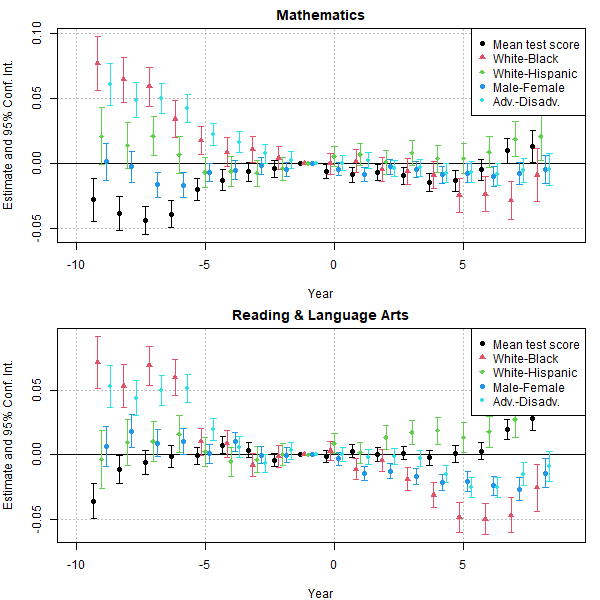
\includegraphics[scale=1]{"../Code & Data/ResultsPlot.pdf"}
	\caption{Dynamic Treatment effects in relative time: FEMA disaster data}
	\label{ResultsPlot}
\end{figure}


For the period of treatment there is a significant\footnote{Significant is used here in the sense that a confidence interval with nominal coverage of 95\% does not include zero, that is a corresponding t-test would reject the null hypothesis of a zero effect at the 5\% level.} effect of natural disasters on the performance in mathematics. The effect size is between just above zero and -0.01 standard deviations. Also, one year after the disaster there is an even larger significant decrease in test scores. For all subsequent periods the effect is not significant. There are some point estimates well below zero, but the uncertainty around those is relatively large. For performance in RLA, there are no significant effects.

Note that the number of observed units decreases with the distance in time from treatment. The reason for this is that in order to experience eight treated years, the county has to experience its first disaster very early. Similarly, it has to receive treatment very late to experience more than five years before treatment. As a result, the uncertainty increases with the distance in time from treatment.

For the subgroups we find some surprising results. Black students seem to perform better in RLA in the medium term after a disaster. That is, there are significantly positive results one to seven years after treatment. The effect sizes are substantial: Seven years after treatment the increase in RLA performance goes up to 0.1 standard deviations. In other words, the average black student sees an increase in performance of up to 0.1 standard deviations of the national reference cohort. Also, hispanic students score significantly lower in mathematics in the year following a disaster.



Positive effects of disasters on performance are not unheard of in the literature. In fact, this is somewhat consistent with the findings by \cite{Sacerdote_2012}. Many students have to switch schools and some may even benefit from attending a higher quality school after the disaster. Black students may disproportionally attend lower quality schools and are therefore more likely to benefit from having to switch schools. 

Figures \ref{ResultsPlotStorm} shows the same graphs based on the storm treatment. The results look very similar. In the period of the storm there is a significant decrease in mathematics scores of up to -0.015 standard deviations. For the years following treatment there are no significant effects.

For female students there is a significant decrease in both subjects in the period of the storm. For RLA we even find a significantly negative effect one year after the storm. Similarly, economically disadvantaged students perform worse in the period of treatment and in RLA one year after treatment. The effect sizes range from barely above zero up to -0.015 or even -0.02 standard deviations. For black and hispanic students we do not find any significant effects of the storm treatment.

\begin{figure}[!h]
	\centering
	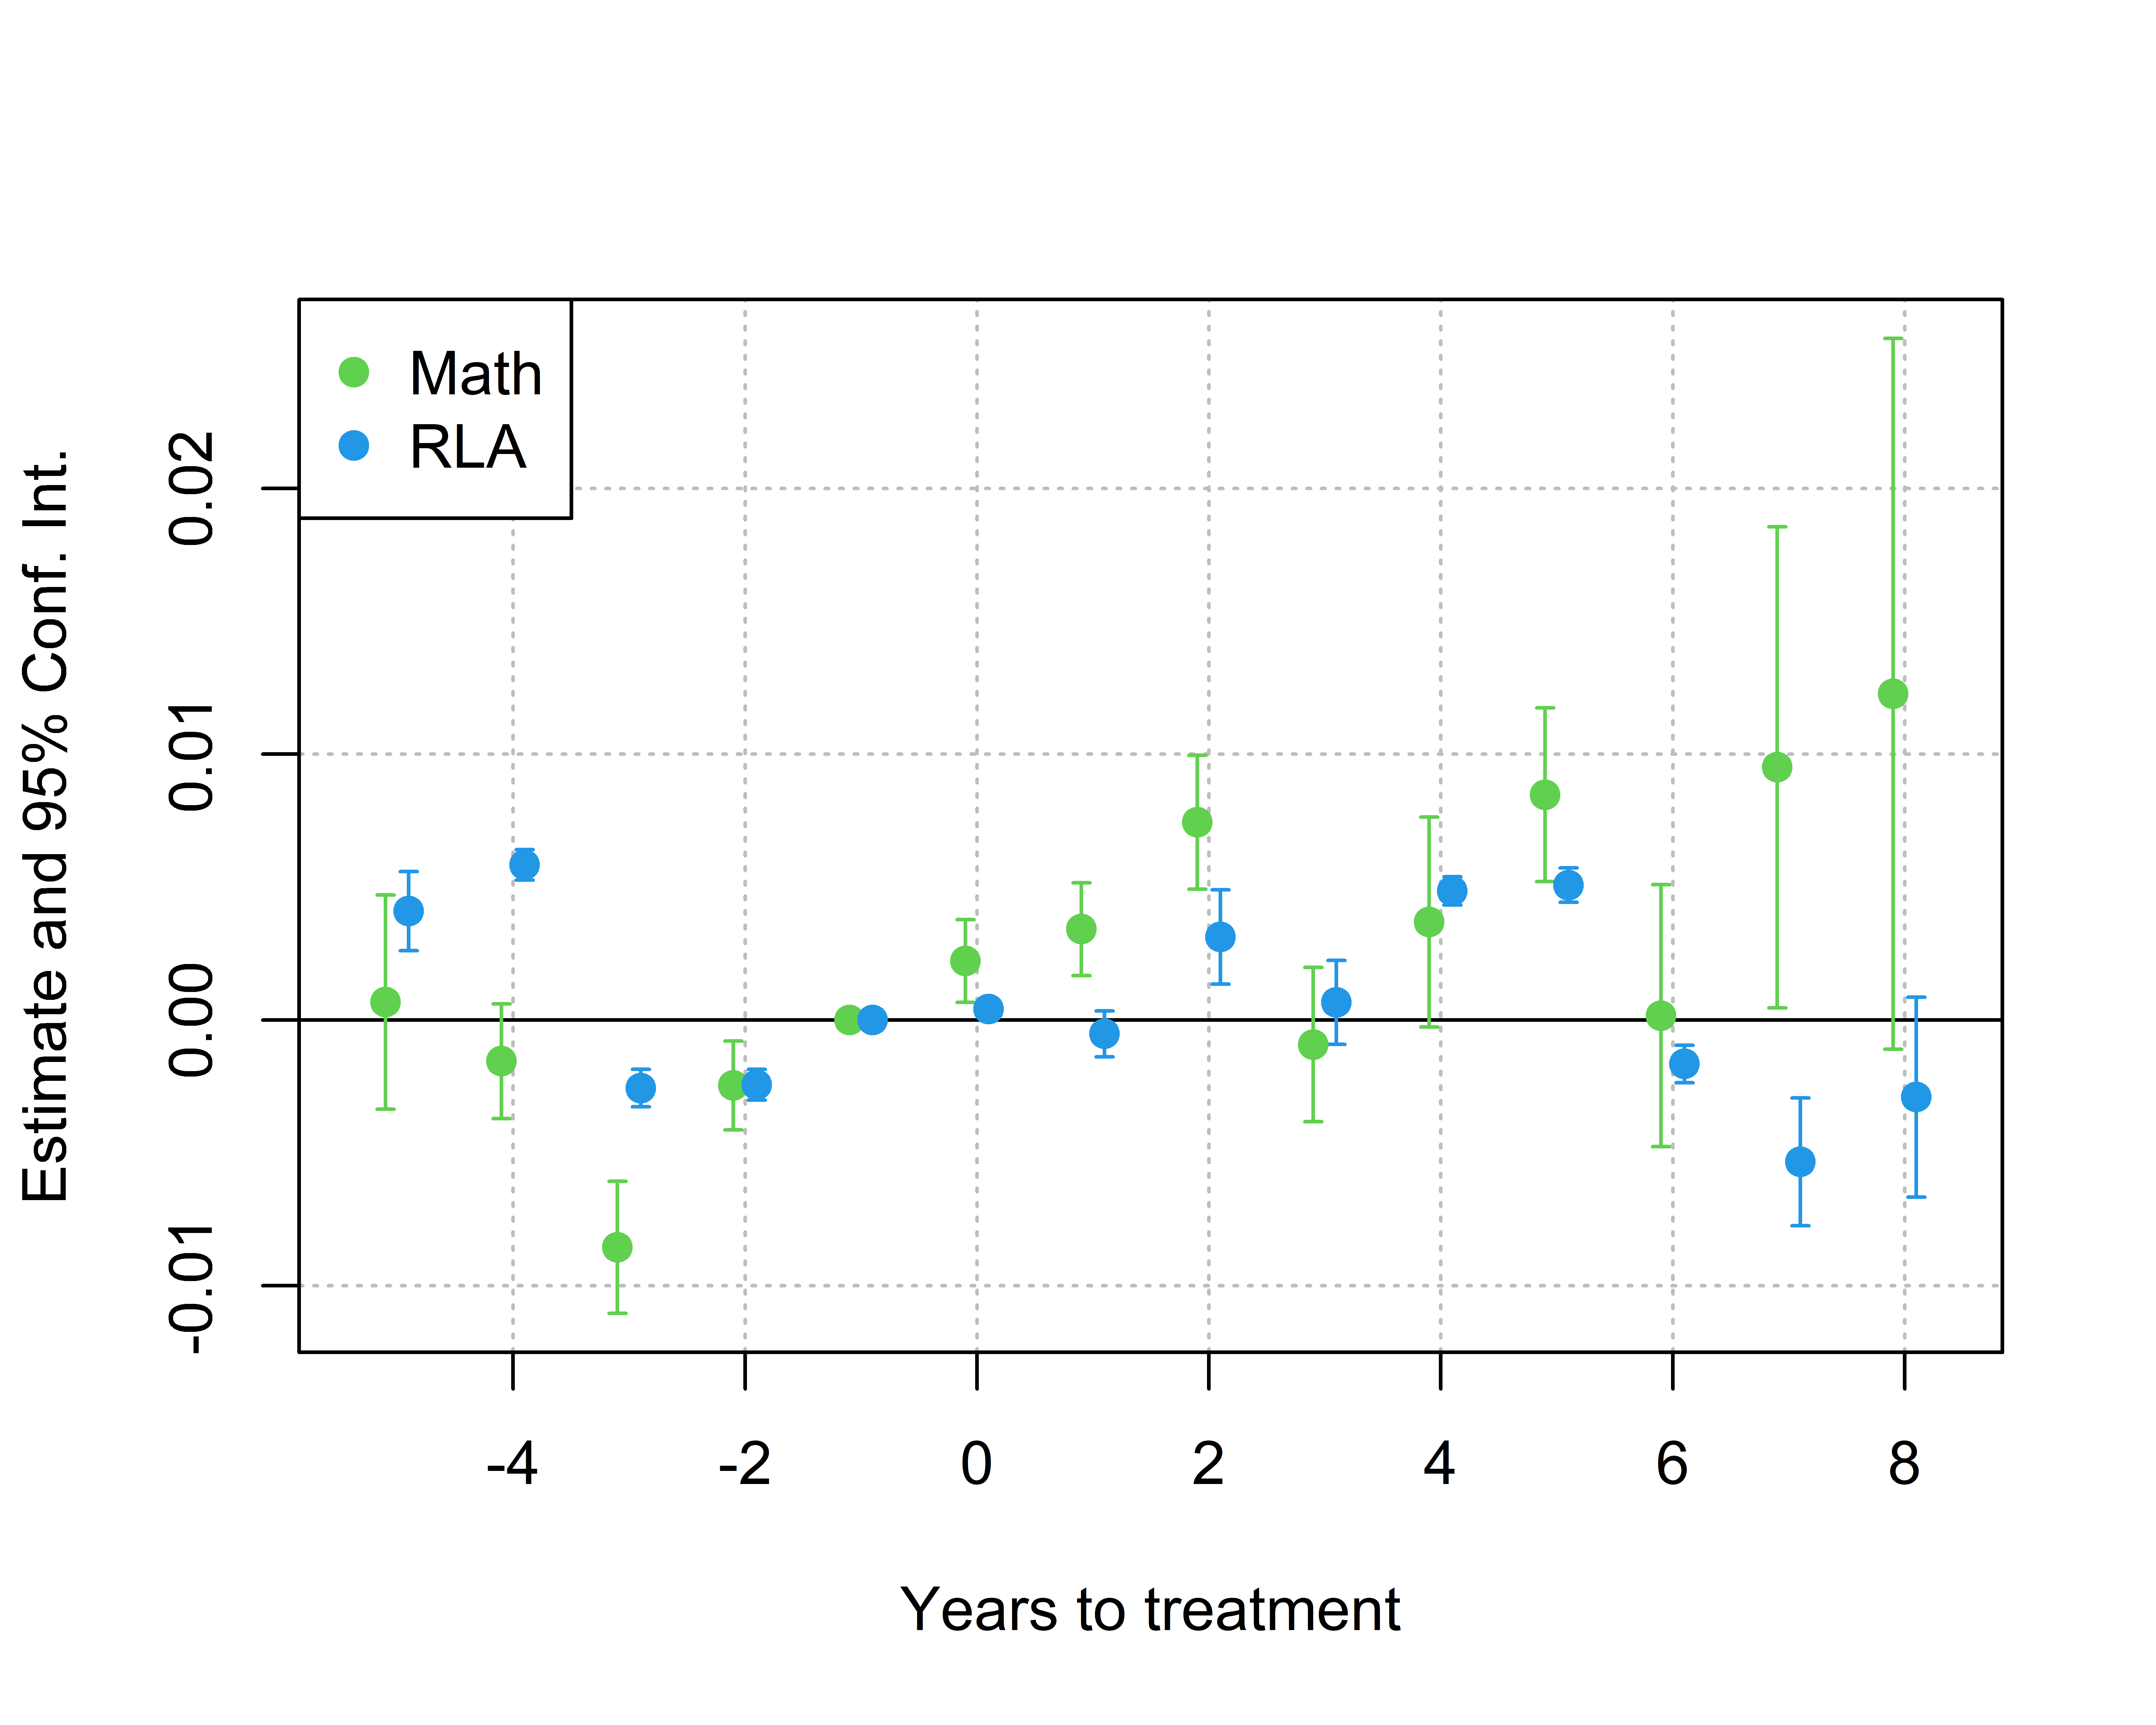
\includegraphics[scale=1]{"../Code & Data/ResultsPlotStorm.pdf"}
	\caption{Dynamic Treatment effects in relative time: NWS storm data}
	\label{ResultsPlotStorm}
\end{figure}


It could be the case that medium- and long-term effects are largely driven by migration. That's why it may be interesting to have a look at the ethnic composition of the counties relative to initial treatment. Figure \ref{EthnicComposition} shows ethnic shares for the treated counties in relative time.

\begin{figure}[!h]
	\centering
	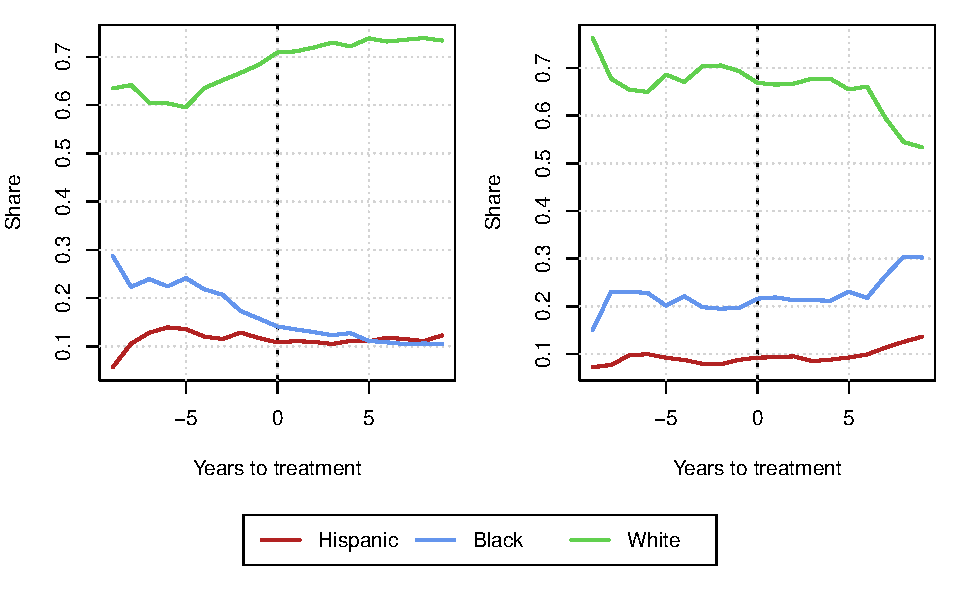
\includegraphics[scale=1]{"../Code & Data/EthnicComposition.pdf"}
	\caption{Aggregated ethnic shares by treatment timing based on FEMA disasters (left) and on NWS storms (right)}
	\label{EthnicComposition}
\end{figure}

In the left panel we see that the share of black students decreases in counties that experienced a disaster. This supports the hypothesis that black students disproportionately switch schools after disasters and may explain the positive long term effect as described above. However, the share of black students already decreases before treatment, so this may not be a causal effect of the disaster.

The same plot based on the NWS storm data shows a different picture. Here, all three shares remain somewhat constant until five years fter treatment. Then the share of black students increases, while the share of white students decreases. This suggests that the migration response to storms may be qualitatively different than the response to other forms of disasters. At least for the storms data this does not seem to be a major driver of the results.

A more in-depth analysis of migration responses to natural disasters and their role in academic achievement is unfortunately not possible with this data. There is some prior research based on individual level data indicating that it does play an important role \citep[for example][]{Sacerdote_2012}. Analyzing migration responses for different types of natural disasters may be a promising area for future research.

Appendix \ref{PowerAna} provides an analysis of the power. For the short-term effects the power is relatively large for plausible true parameter values. Thus, we can be relatively certain that non-significant results are true negatives.



\section{Conclusion} \label{Conclusion}

The main contribution of this paper is estimating dynamic treatment effects for natural disasters on academic achievement. In most specifications, we find negative short-term effects on the average mathematics test scores. Black and hispanic students, however, do not experience these. Based on the FEMA declarations data, there are positive long-term effects in reading achievement. With the NWS storms data, this effect is only visible among white students.

Some of these results may be driven by migration. Shares of hispanic and black students tend to decrease around the time of disasters, at least based on the FEMA declarations. This might explain why they do not experience such pronounced short-term decreases in test scores. Yet, this is somewhat speculative. For a more detailed analysis of student mobility following a disaster, individual level data would be preferable.

Based on temperature data, we analyze the effect of heat exposure on academic performance. We find some significantly negative effects. Hispanic students seem to be especially affected by excessive heat. These discrepancies are likely driven by differing access to air-conditiong. Providing widespread access to air-conditioning can be an effective policy option to prevent such negative effects.

Both the frequency and the severity of natural disasters will increase in the future. Similarly, heat exposure will substantially increase over the next decades. Minimizing the negative effects will be essential in order not to jeopardize children's success at school. Policymakers must focus on mitigating climate change through effective action. However, some effects will only be able to be mitigated to a very limited extent. That is where effective relief measures after a disaster are needed.






% appendix
\appendix

\section{Additional Results} \label{AppendixA}

\subsection{Logistic regression for assistance applications}

Below we report logistic regression results for the applicant status, that is whether a county applied for federal disaster assistance based on the Public Assistance Applicants Program Deliveries data. This is regressed on a few variables, including the share of democratic votes in the 2016 election. The other independent variables are also from 2016.

Similarly, the declaration status, that is whether a county had any natural disasters declared during the 2009 to 2018 period. This is regressed on the share of democratic votes in the 2008 election and the set of same control variables.


\begin{table}[htbp]
   \centering
   \caption{\label{ResultsLogit} Determinants of Assistance Application}
   \begin{tabular}{lc}
      \tabularnewline\midrule\midrule
      Dependent Variable:        & Applicant\\
      Model:                     & (1)\\
      \midrule \emph{Variables} &  \\
      (Intercept)                & -3.622\\
                                 & (3.723)\\
      Share of democratic voters & -0.8362$^{**}$\\
                                 & (0.3469)\\
      Median Income (logs)       & 0.2939\\
                                 & (0.3331)\\
      Poverty Rate               & 4.033$^{**}$\\
                                 & (1.575)\\
      Share of single mothers    & 4.068$^{***}$\\
                                 & (1.144)\\
      \midrule \emph{Fit statistics} &  \\
      Observations               & 2,882\\
      Squared Correlation        & 0.02306\\
      Pseudo R$^2$               & 0.01966\\
      BIC                        & 3,724.7\\
      \midrule\midrule\multicolumn{2}{l}{\emph{IID standard-errors in parentheses}}\\
      \multicolumn{2}{l}{\emph{Signif. Codes: ***: 0.01, **: 0.05, *: 0.1}}\\
   \end{tabular}
\end{table}





\section{Pre-Treatment Trends} \label{PreTrends}

Here we display plots of aggregated pre-treatment trends to justify the parallel trends assumption. Mean test scores are aggregated by cohort (year of first treatment) and relative time to treatment, and never treated units act as the control group. Figure \ref{PreTrendsMath} and \ref{PreTrendsRLA} show the results for mathematics and RLA respectively. We only display these plots for overall test scores and not for subgroups. However, the plots for the subgroups look very similar.


\begin{figure}[!h]
	\centering
	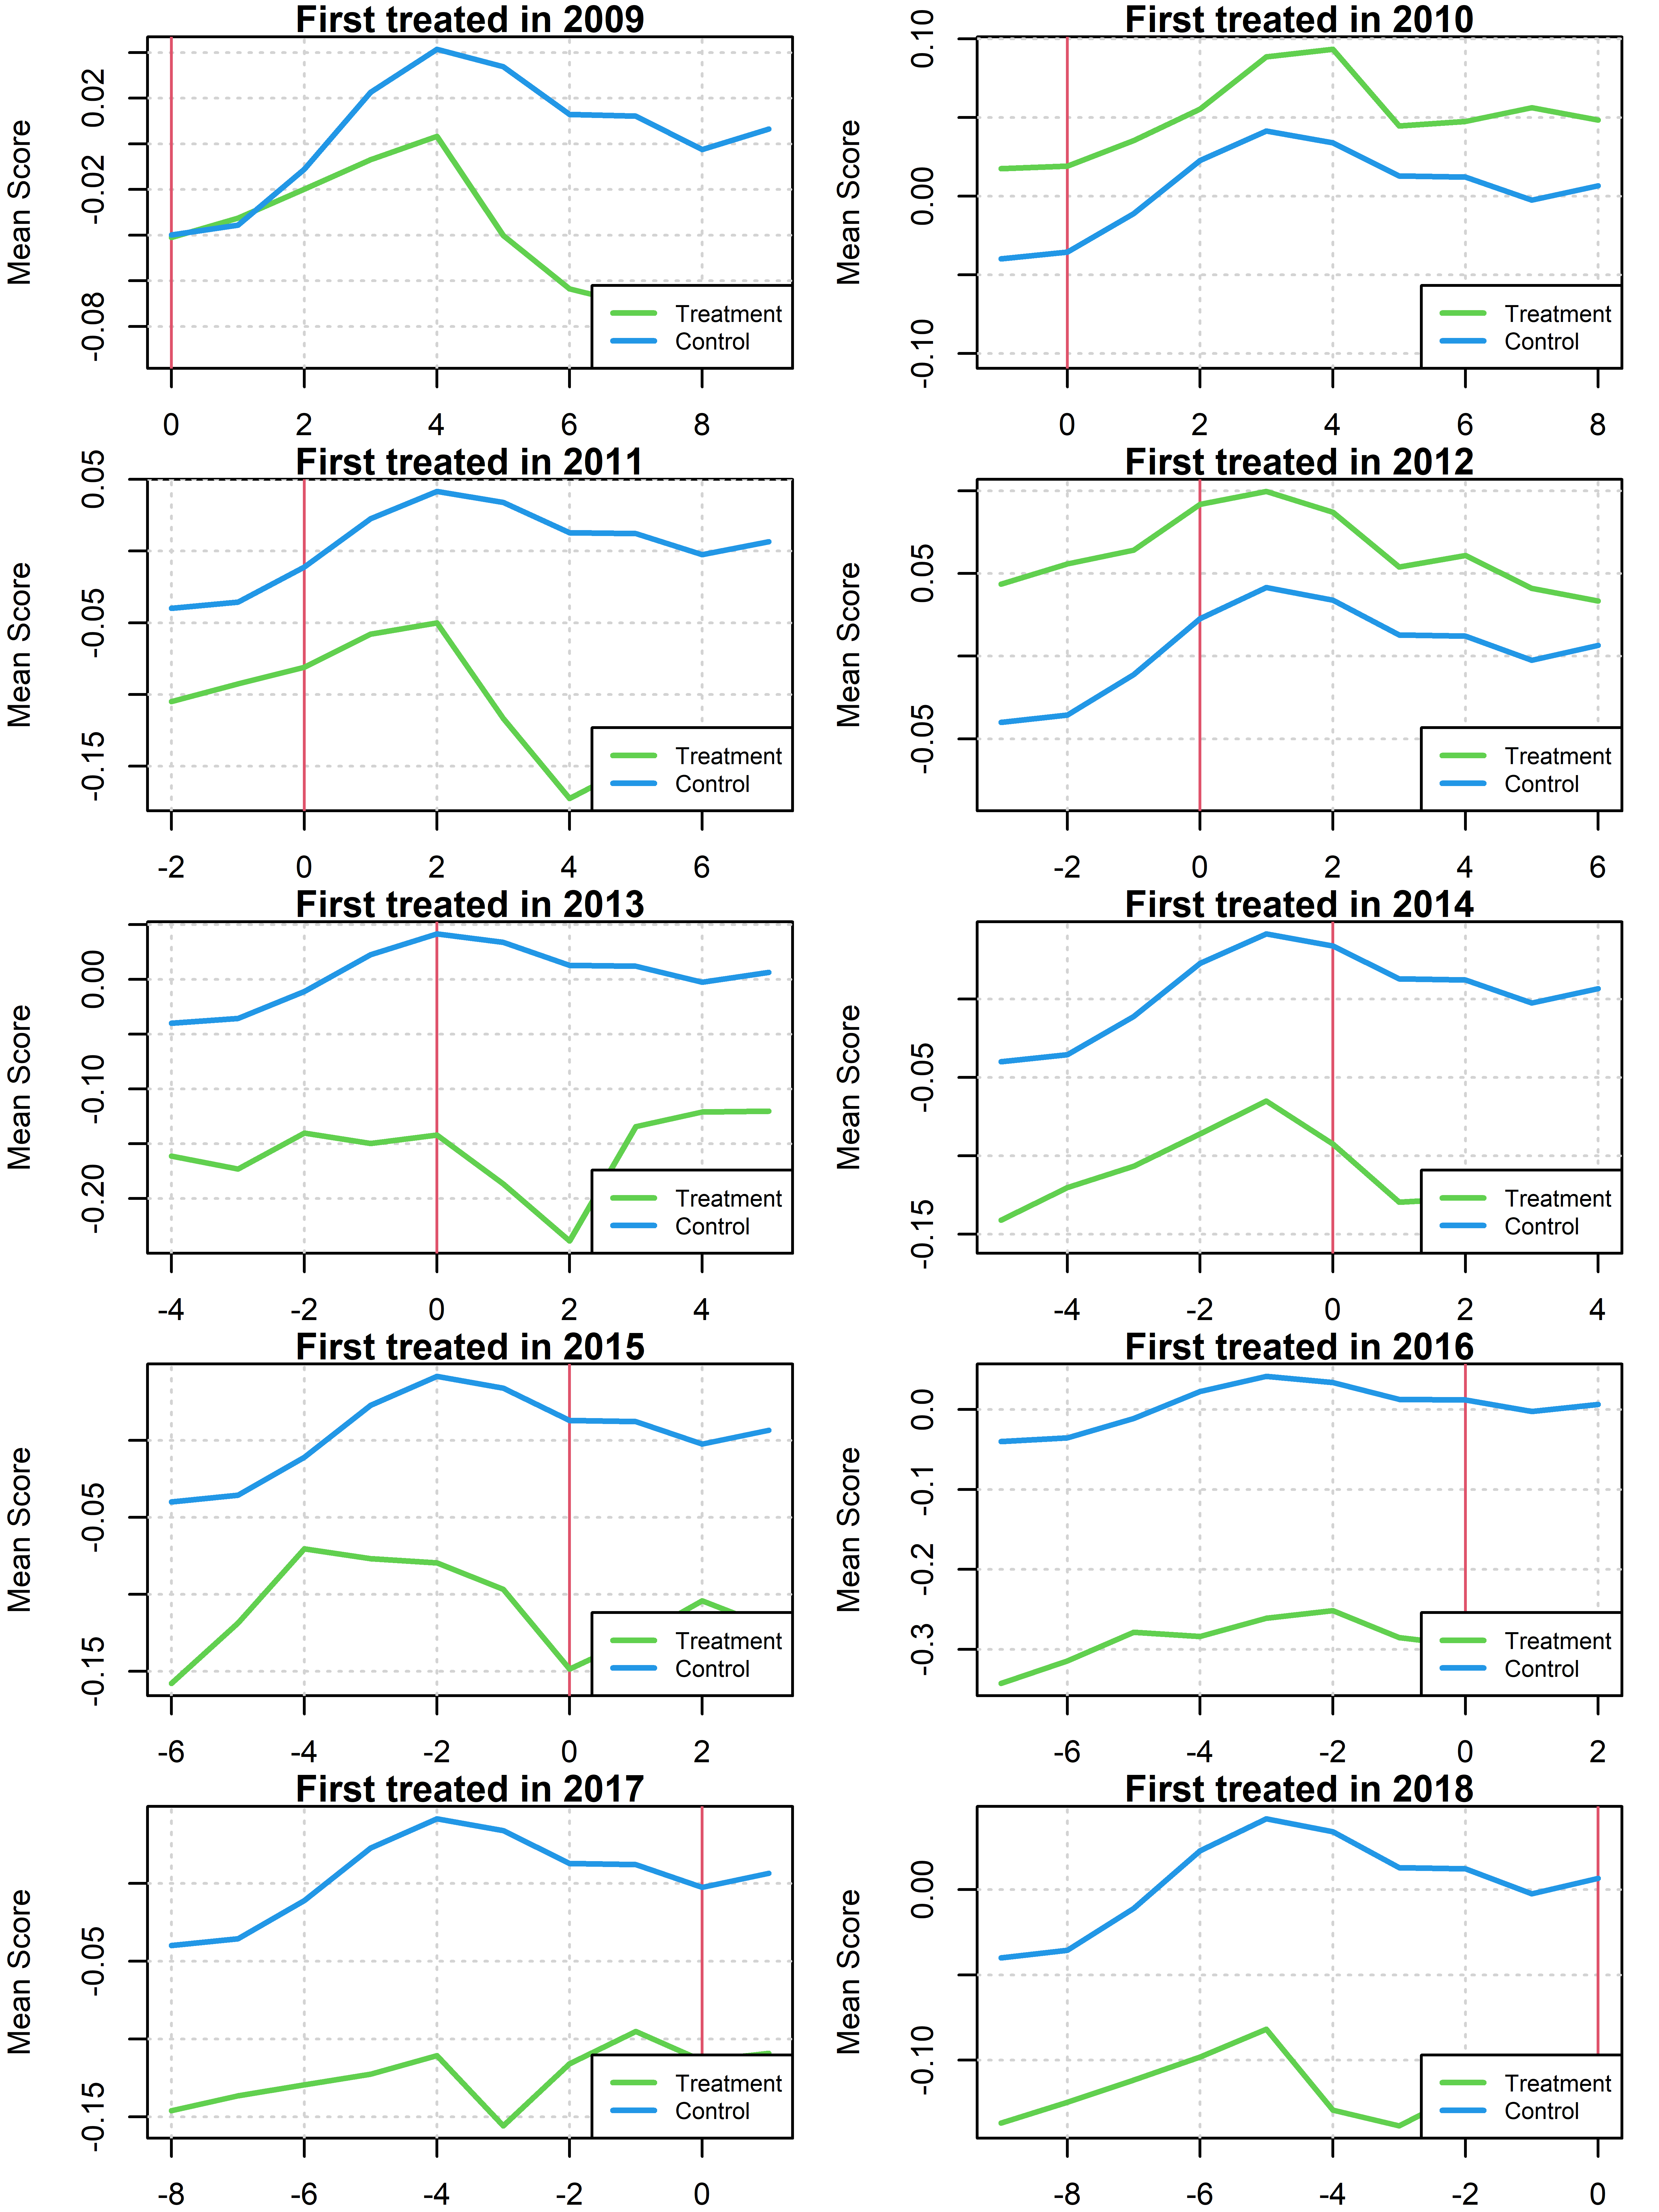
\includegraphics[scale=1]{"../Code & Data/ParTrendsPlotMathematics.png"}
	\caption{Pre trends for aggregated mean scores in mathematics}
	\label{PreTrendsMath}
\end{figure}

\begin{figure}[!h]
	\centering
	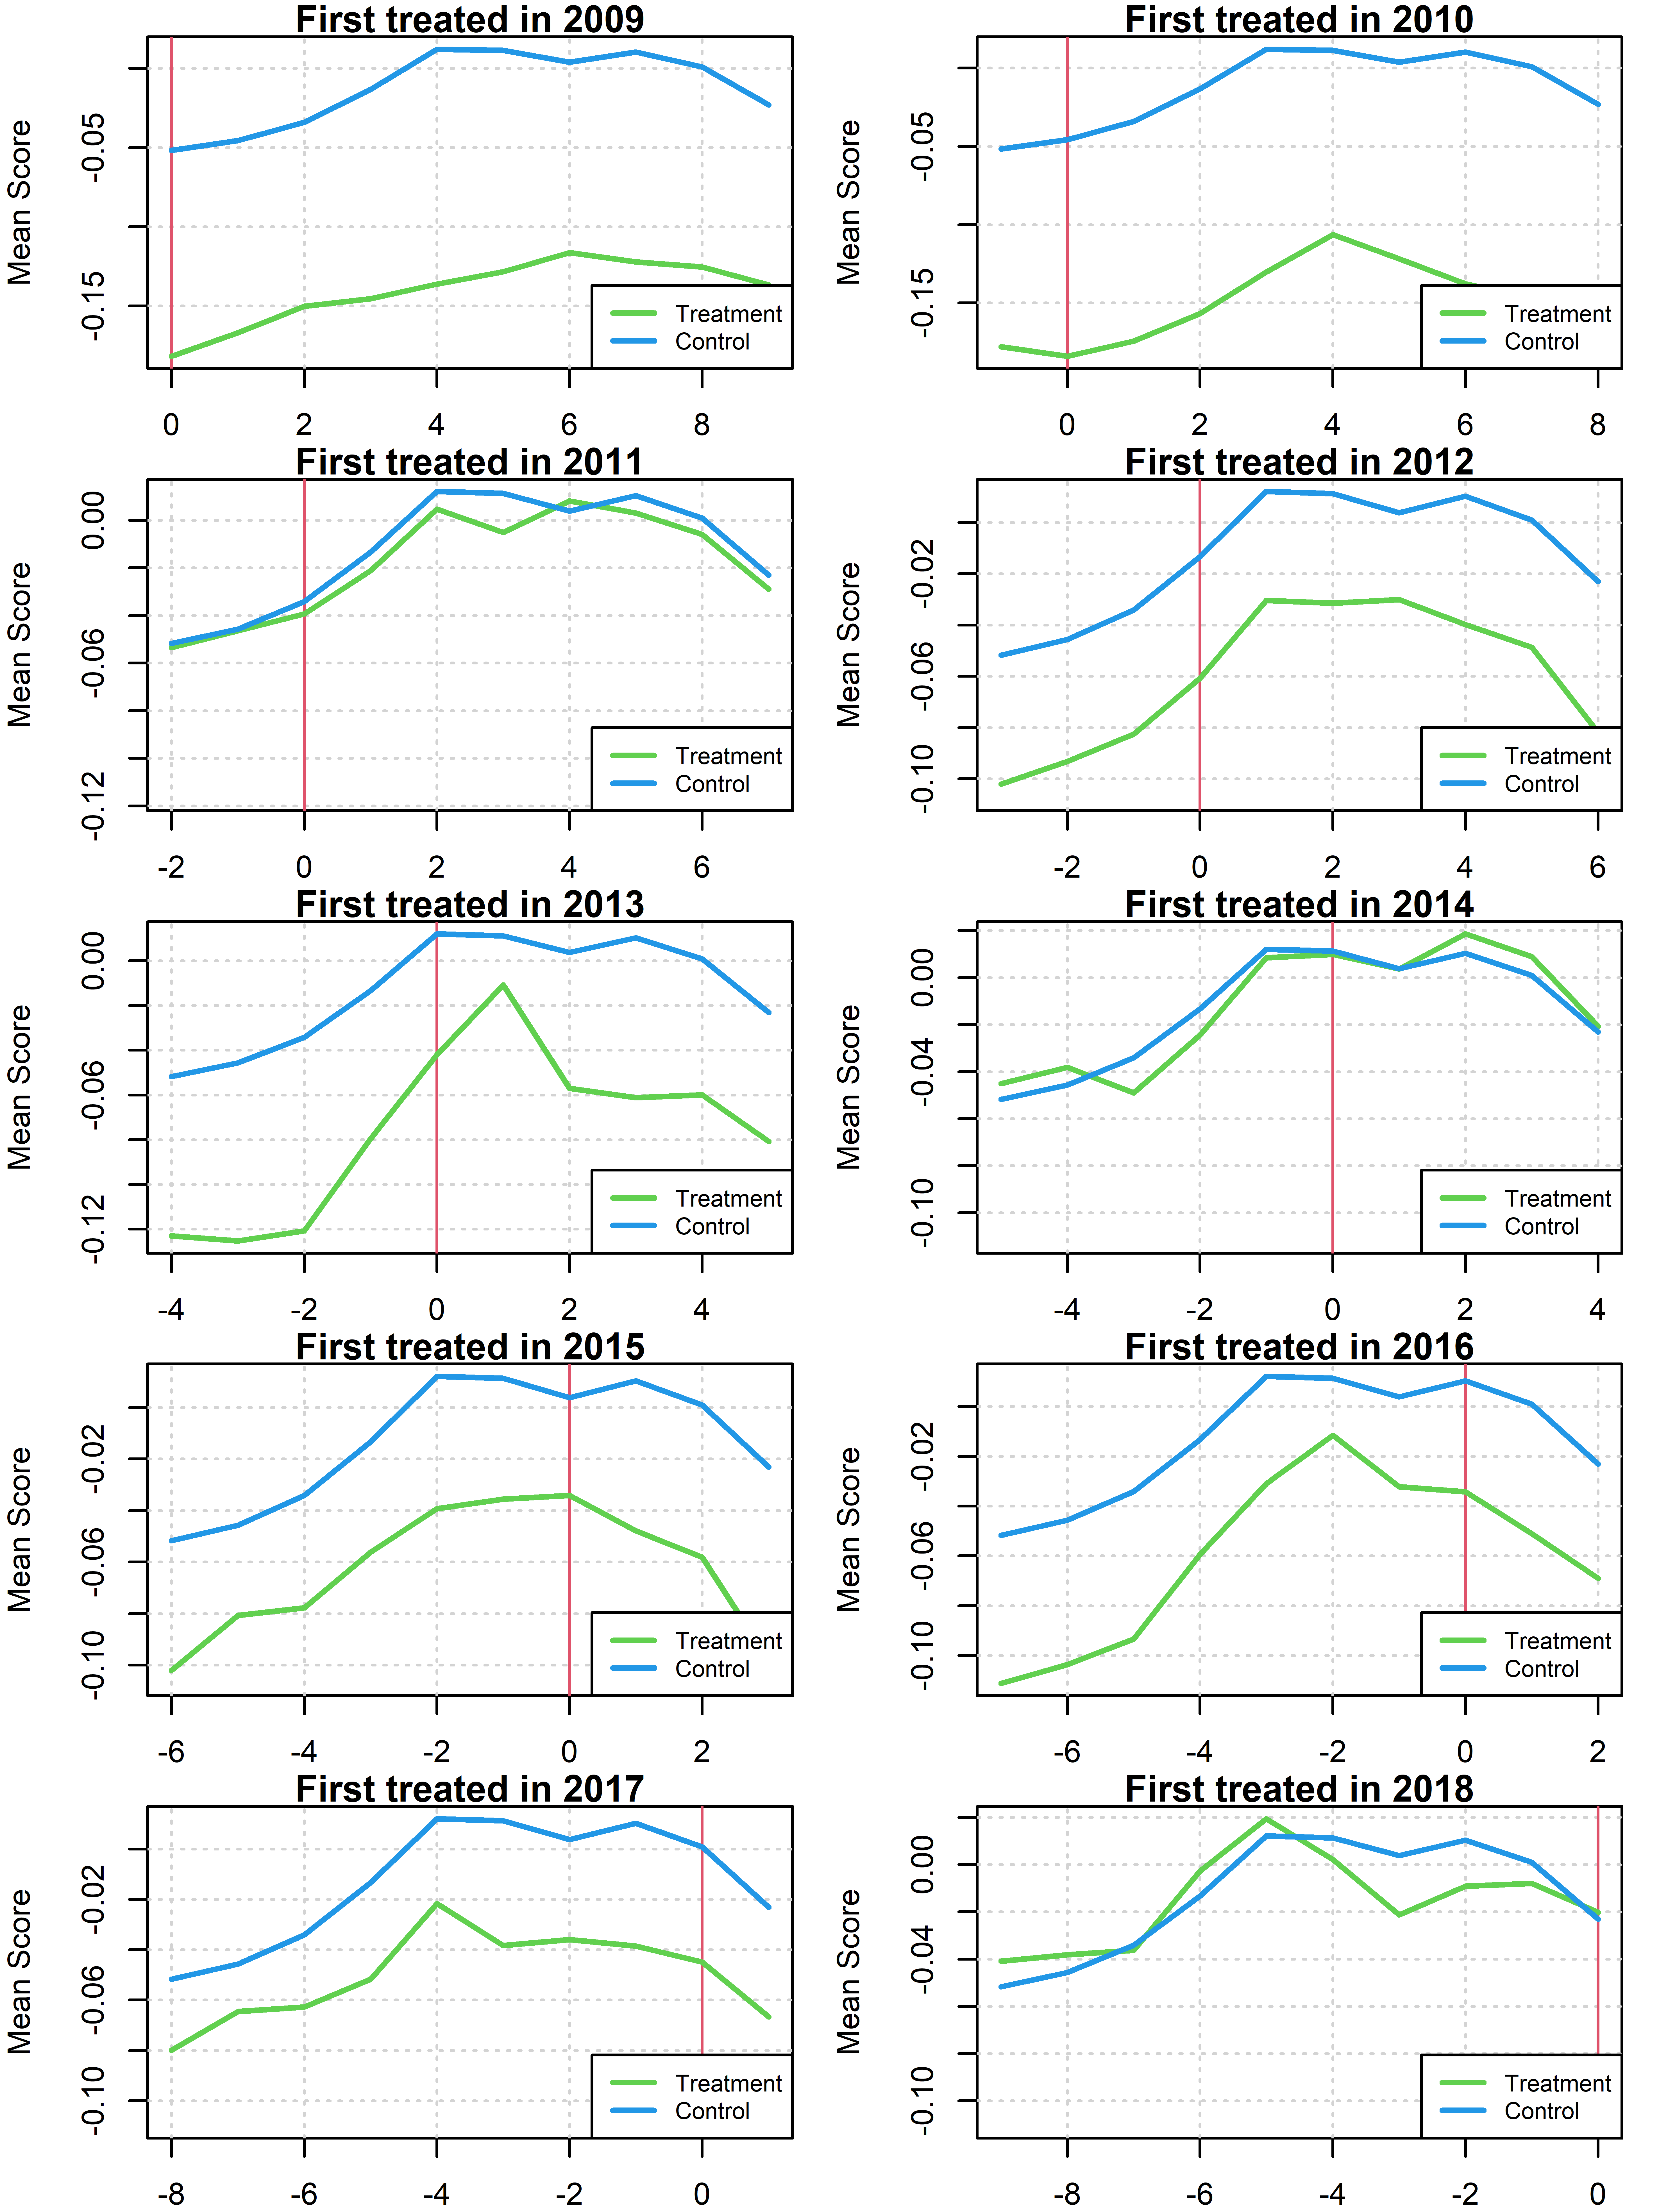
\includegraphics[scale=1]{"../Code & Data/ParTrendsPlotRLA.png"}
	\caption{Pre trends for aggregated mean scores in RLA}
	\label{PreTrendsRLA}
\end{figure}





% bibliography
\bibliographystyle{apalike}
\bibliography{references}

\end{document}          



